
\documentclass[a4paper,12pt]{article}
\usepackage[utf8]{inputenc}
\usepackage[a4paper,
            bindingoffset=0.2in,
            left=1in,
            right=1in,
            top=1in,
            bottom=1in,
            footskip=.25in]{geometry}


%###############################################################################

%\input{~/layout/global_layout}


%###############################################################################

% packages begin

\usepackage[
  backend=biber,
  sortcites=true,
  style=alphabetic,
  eprint=true,
  backref=true
]{biblatex}
\addbibresource{bibliography.bib}

\usepackage{euscript}[mathcal]
% e.g. \mathcal{A} for fancy letters in mathmode
\usepackage{amsmath,amssymb,amstext,amsthm}

\usepackage{mdframed}
\newmdtheoremenv[nobreak=true]{problem}{Problem}[subsection]
\newmdtheoremenv[nobreak=true]{claim}{Claim}[subsection]
\newtheorem{definition}{Definition}[subsection]
\newtheorem{lemma}{Lemma}[claim]
\newtheorem{plemma}{Lemma}[problem]

\usepackage{mathtools}
\DeclarePairedDelimiter\ceil{\lceil}{\rceil}
\DeclarePairedDelimiter\floor{\lfloor}{\rfloor}

\usepackage{enumerate}
\usepackage[pdftex]{graphicx}
\usepackage{subcaption}
% 'draft' für schnelleres rendern mitübergeben -> [pdftex, draft]
% dadruch wird nicht das bild mitgerendered, sondern nur ein kasten mit bildname -> schont ressourcen

\usepackage{hyperref}

\usepackage{tikz}
\usetikzlibrary{arrows,automata,matrix,positioning,shapes}

% for adding non-formatted text to include source-code
\usepackage{listings}
\lstset{language=Python,basicstyle=\footnotesize}
% z.B.:
% \lstinputlisting{source_filename.py}
% \lstinputlisting[lanugage=Python, firstline=37, lastline=45]{source_filename.py}
%
% oder
%
% \begin{lstlisting}[frame=single]
% CODE HERE
%\end{lstlisting}
\usepackage{algorithm}
\usepackage{algpseudocode}

\usepackage{wasysym}

\usepackage{titling}
\usepackage{titlesec}
\usepackage[nocheck]{fancyhdr}
\usepackage{lastpage}

\usepackage{kantlipsum}
\usepackage[colorinlistoftodos,prependcaption,textsize=tiny]{todonotes}

% packages end
%###############################################################################

\pretitle{% add some rules
  \begin{center}
    \LARGE\bfseries
} %, make the fonts bigger, make the title (only) bold
\posttitle{%
  \end{center}%
  %\vskip .75em plus .25em minus .25em% increase the vertical spacing a bit, make this particular glue stretchier
}
\predate{%
  \begin{center}
    \normalsize
}
\postdate{%
  \end{center}%
}

\titleformat*{\section}{\Large\bfseries}
\titleformat*{\subsection}{\large\bfseries}
\titleformat*{\subsubsection}{\normalsize\bfseries}

\titleformat*{\paragraph}{\Large\bfseries}
\titleformat*{\subparagraph}{\large\bfseries}

%###############################################################################
% TODO define Headers and Fotter

\pagestyle{fancy}
\fancyhf{}
% l=left, c=center, r=right; e=even_pagenumber, o=odd_pagenumber; h=header, f=footer
% example: [lh] -> left header, [lof,ref] -> fotter left when odd, right when even
%\fancyhf[lh]{}
%\fancyhf[ch]{}
%\fancyhf[rh]{}
%\fancyhf[lf]{}
\fancyhf[cf]{\footnotesize Page \thepage\ of \pageref*{LastPage}}
%\fancyhf[rf]{}
\renewcommand{\headrule}{} % removes horizontal header line

% Fotter options for first page

\fancypagestyle{firstpagestyle}{
  \renewcommand{\thedate}{\textmd{}} % removes horizontal header line
  \fancyhf{}
  \fancyhf[lh]{\ttfamily M.Sc. Computer Science\\KTH Royal Institute of Technology}
  \fancyhf[rh]{\ttfamily Period 3\\\today}
  \fancyfoot[C]{\footnotesize Page \thepage\ of \pageref*{LastPage}}
  \renewcommand{\headrule}{} % removes horizontal header line
}
%###############################################################################
% Todo: define Title

\title{
  \normalsize{DD2358 VT25 Introduction to}\\
  \normalsize{High Performance Computing}\\
  \large{Assignment 2}\\
}
\author{
  \small Lennart Herud\\[-0.75ex]
%  \footnotesize\texttt{MN: }\\[-1ex]
  \scriptsize\texttt{herud@kth.se}
  \and
    \small Paul Mayer\\[-0.75ex]
%  \footnotesize\texttt{MN: }\\[-1ex]
  \scriptsize\texttt{pmayer@kth.se}
  \and
    \small Adrian Sušec\\[-0.75ex]
%  \footnotesize\texttt{MN: }\\[-1ex]
  \scriptsize\texttt{susec@kth.se}
  \and
  \small Rishi Vijayvargiya\\[-0.75ex]
%  \footnotesize\texttt{MN: }\\[-1ex]
  \scriptsize\texttt{rishiv@kth.se}
}
\date{}

%###############################################################################
% define Commands

\newcommand{\N}{\mathbb{N}}
\newcommand{\R}{\mathbb{R}}
\newcommand{\Z}{\mathbb{Z}}
\newcommand{\I}{\mathbb{I}}

\newcommand{\E}{\mathbb{E}}
\newcommand{\Prob}{\mathbb{P}}

\renewcommand{\epsilon}{\varepsilon}

% Todo: Set Counter to Excercise Sheet Number
%\setcounter{section}{1}
%\setcounter{subsection}{1}

%###############################################################################
%###############################################################################

\begin{document}
\maketitle
\thispagestyle{firstpagestyle}

% \tableofcontents
\listoftodos

\vspace{1em}

%---
%
\section*{Prefix}
\todo[inline]{Make sure title and headers are correctly changed!}
\todo[inline]{Change counter to match excercise sheet}

% content begin
%

\section{PyTest with the Julia Set Code}
\section{Python DGEMM Benchmark Operation}
\section{Experiment with the Python Debugger}
\section{Bonus: Game of Life}
For this task, we examined the code for \textit{Game of Life} found at this location: \url{https://github.com/electronut/pp/blob/master/conway/conway.py}. The working directory for our assignment code referenced in this section is the \verb|bonus/| directory found at this location: \url{https://github.com/paulmyr/DD2358-HPC25/tree/master/02_hpcds/bonus}
\subsection{B.1: Linting and Documentation}
We ran \verb|pylint| on the default \verb|conway.py| file above, and got output that was mostly comprised of warnings/convention/refactor related information. To fix these issues, we used the \verb|black| auto-formatter on the default \verb|conway.py| file, and amended some of these issues (such as missing docstring for a function, or snake-case conformity) manually. Afterwards, only one issue was remaining in the default \verb|conway.py| file -- which had to do with the unused variable \verb|frame_num| for the function \verb|update|. This was left as is, since we believe this was used by the animation function of \verb|matplotlib| to visualize the grid. Information on the output of \verb|pylint| on the default \verb|conway.py| file can be found in the \verb|misc/linting_outputs.txt| file in the repository. 

To generate the documentation, we used the \verb|sphinx| tool on the \verb|conway.py| file after it was modified above to conform to as many python standards as possible (according to \verb|pylint|). The generated documentation can be accessed by clicking on the \verb|docs/html/index.html| page in the working directory for the bonus. Help of this useful tutorial on the \verb|sphinx| tool was taken to generate the documentation: \url{https://www.youtube.com/watch?v=BWIrhgCAae0} (including steps such as modifying the \verb|docs/source/conf.py| file, or generating the required \verb|reStructuredText| (ie, files with extension \verb|rst|) files. An example of clicking on the \verb|conway module| after opening the \verb|docs/html/index.html| page can be seen below

\begin{figure}[h!]
  \centering
  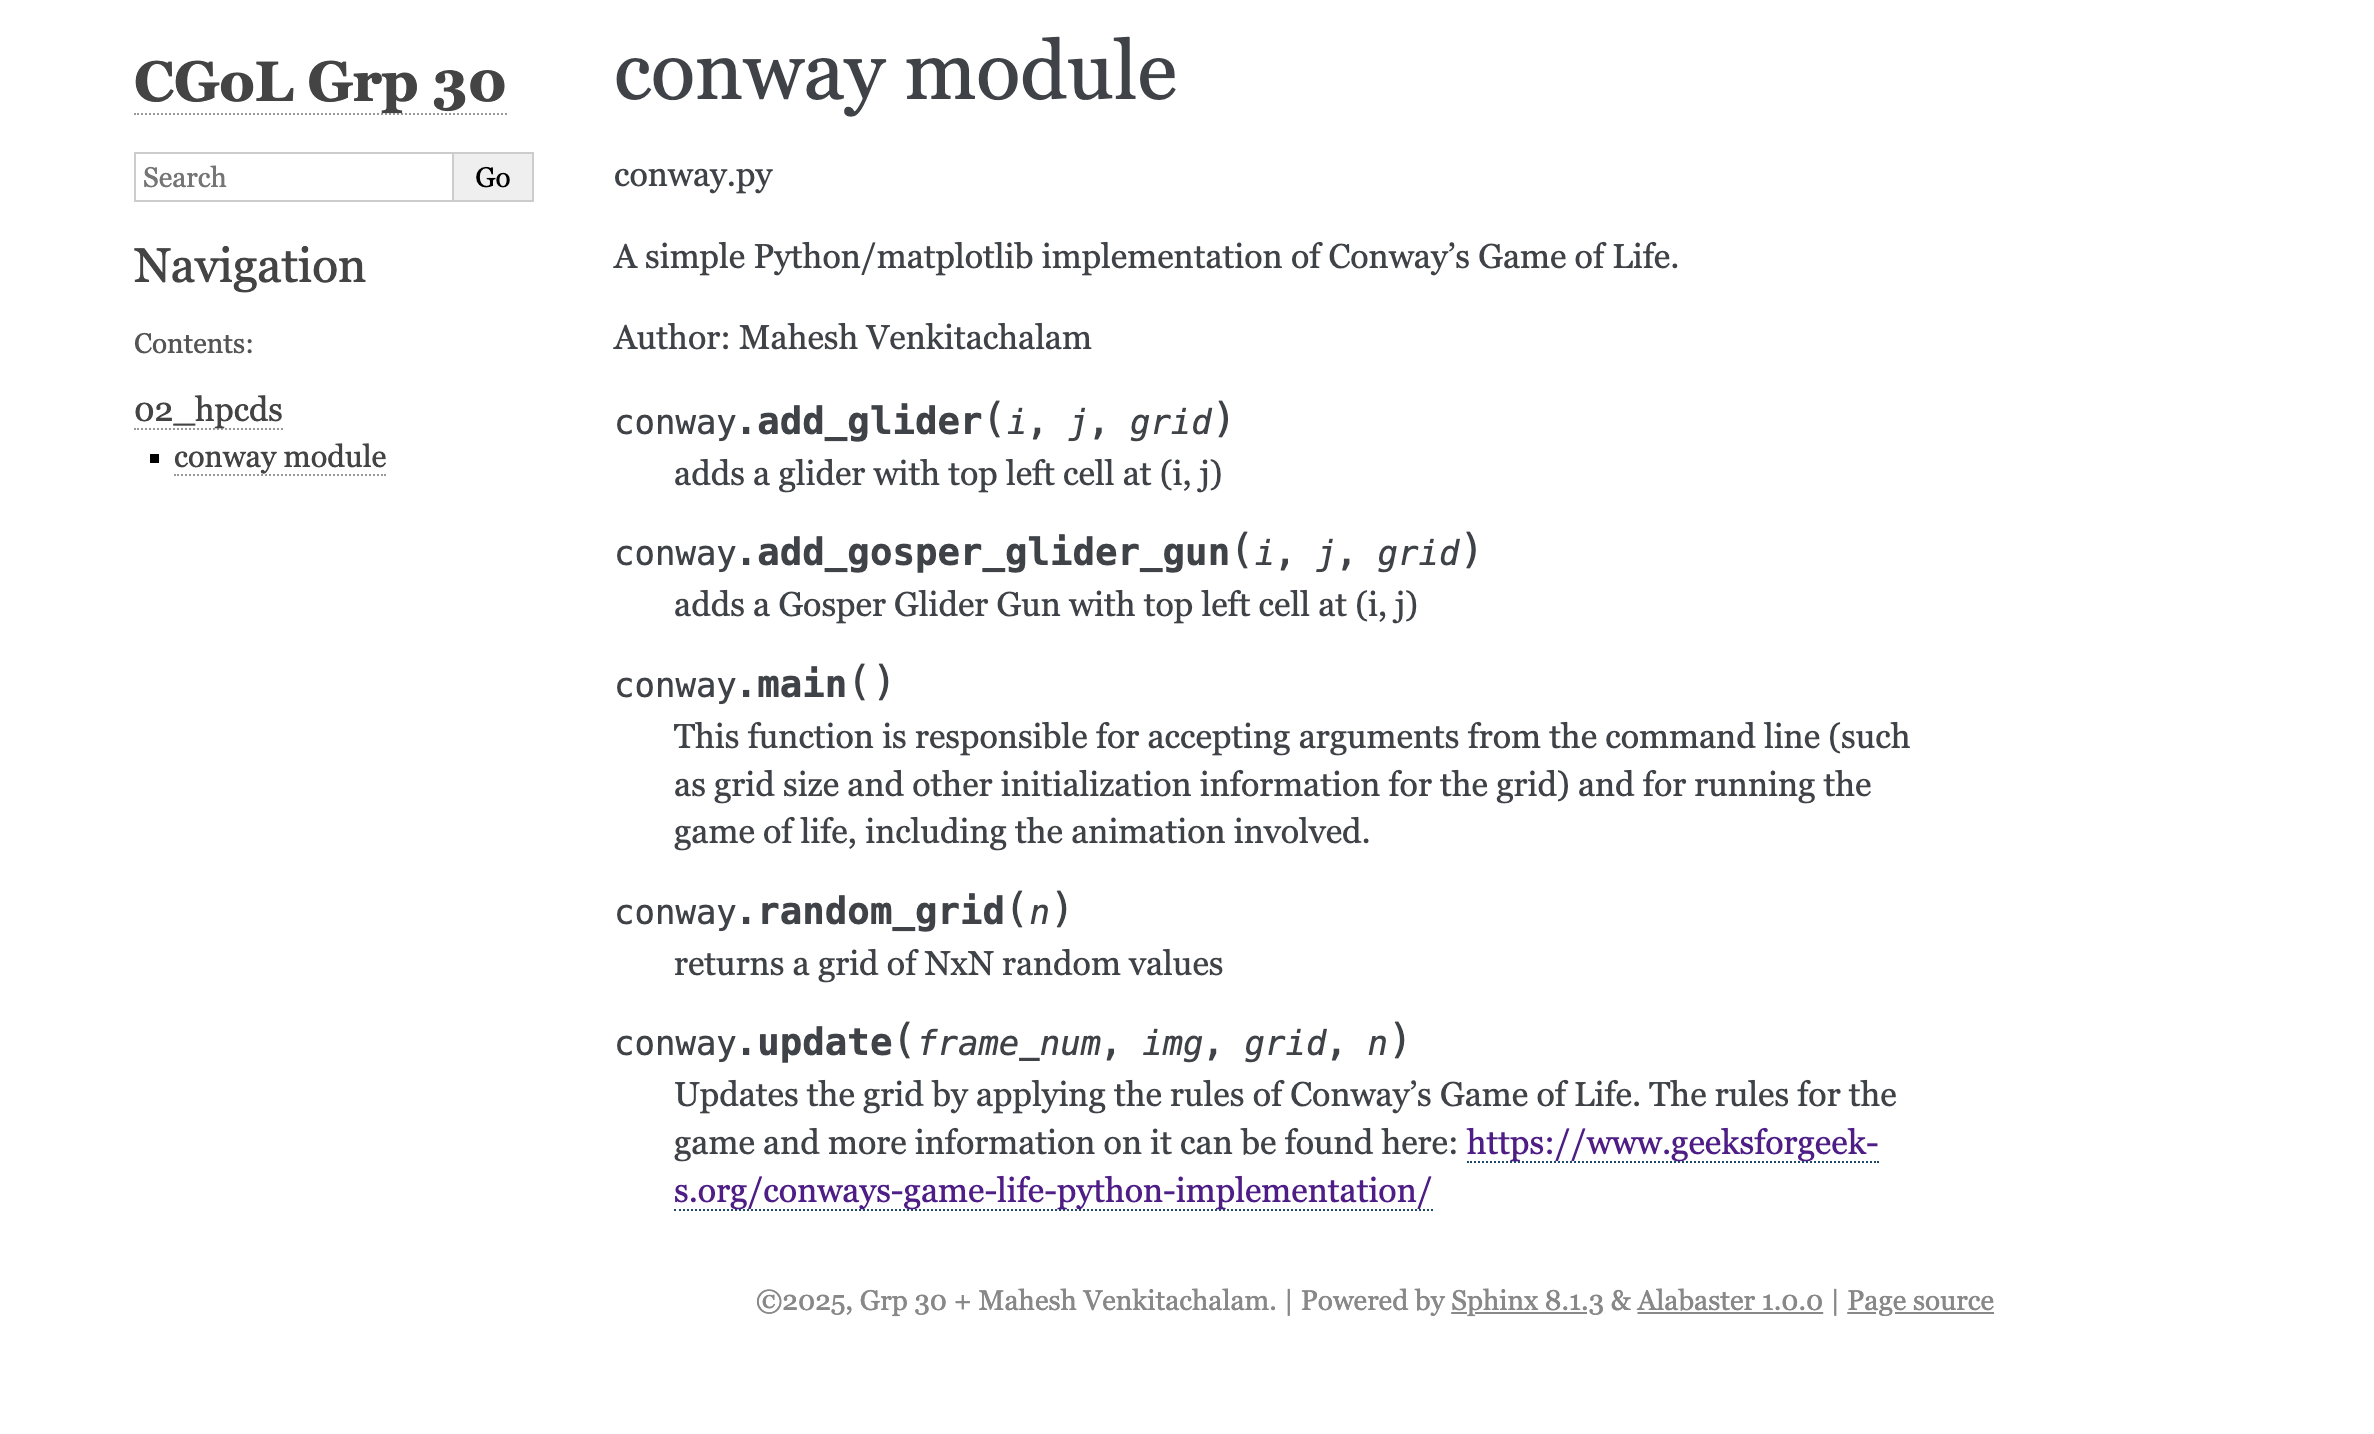
\includegraphics[width=\textwidth]{images/conway_documentation_example.png}
  \caption{Documentation for the Default conway.py File}
  \label{fig:conway_docs}
\end{figure}

Note that we only generated this documentation when only the default \verb|conway.py| file was present (as this was a part preceding the later steps of the Bonus exercise). Thus, only documentation on  the original \verb|conway.py| file (after fixing most of the linting issues) can be found on the docs generated by \verb|sphinx|. The same applies for running \verb|pylint| and \verb|black| -- these commands were only ran on the original \verb|conway.py| file (not any other files present in the repo or used in this bonus section).

\subsection{B.2: Execution Time and Plot}
\subsection{B.3: Profiling Existing Code}
\subsection{B.4: Optimization and Results}
\section{Appendix}

% content end
%###############################################################################

% TODO: bibliograpghy when needed
% \printbibliography

\end{document}